\section{Learning Control-oriented Latent Dynamics from Pixels}\label{sec:learning_latent_space_dynamics}
We now move towards learning latent dynamical models based on \gls{CON} and \gls{CFA-CON}.
% , which we will leverage later in Sec~\ref{sec:latent_space_control} for model-based control. 
\glspl{CON} are an ideal fit for learning latent dynamics as they guarantee that the latent states stay bounded. 

\begin{figure}[t]
    \centering
    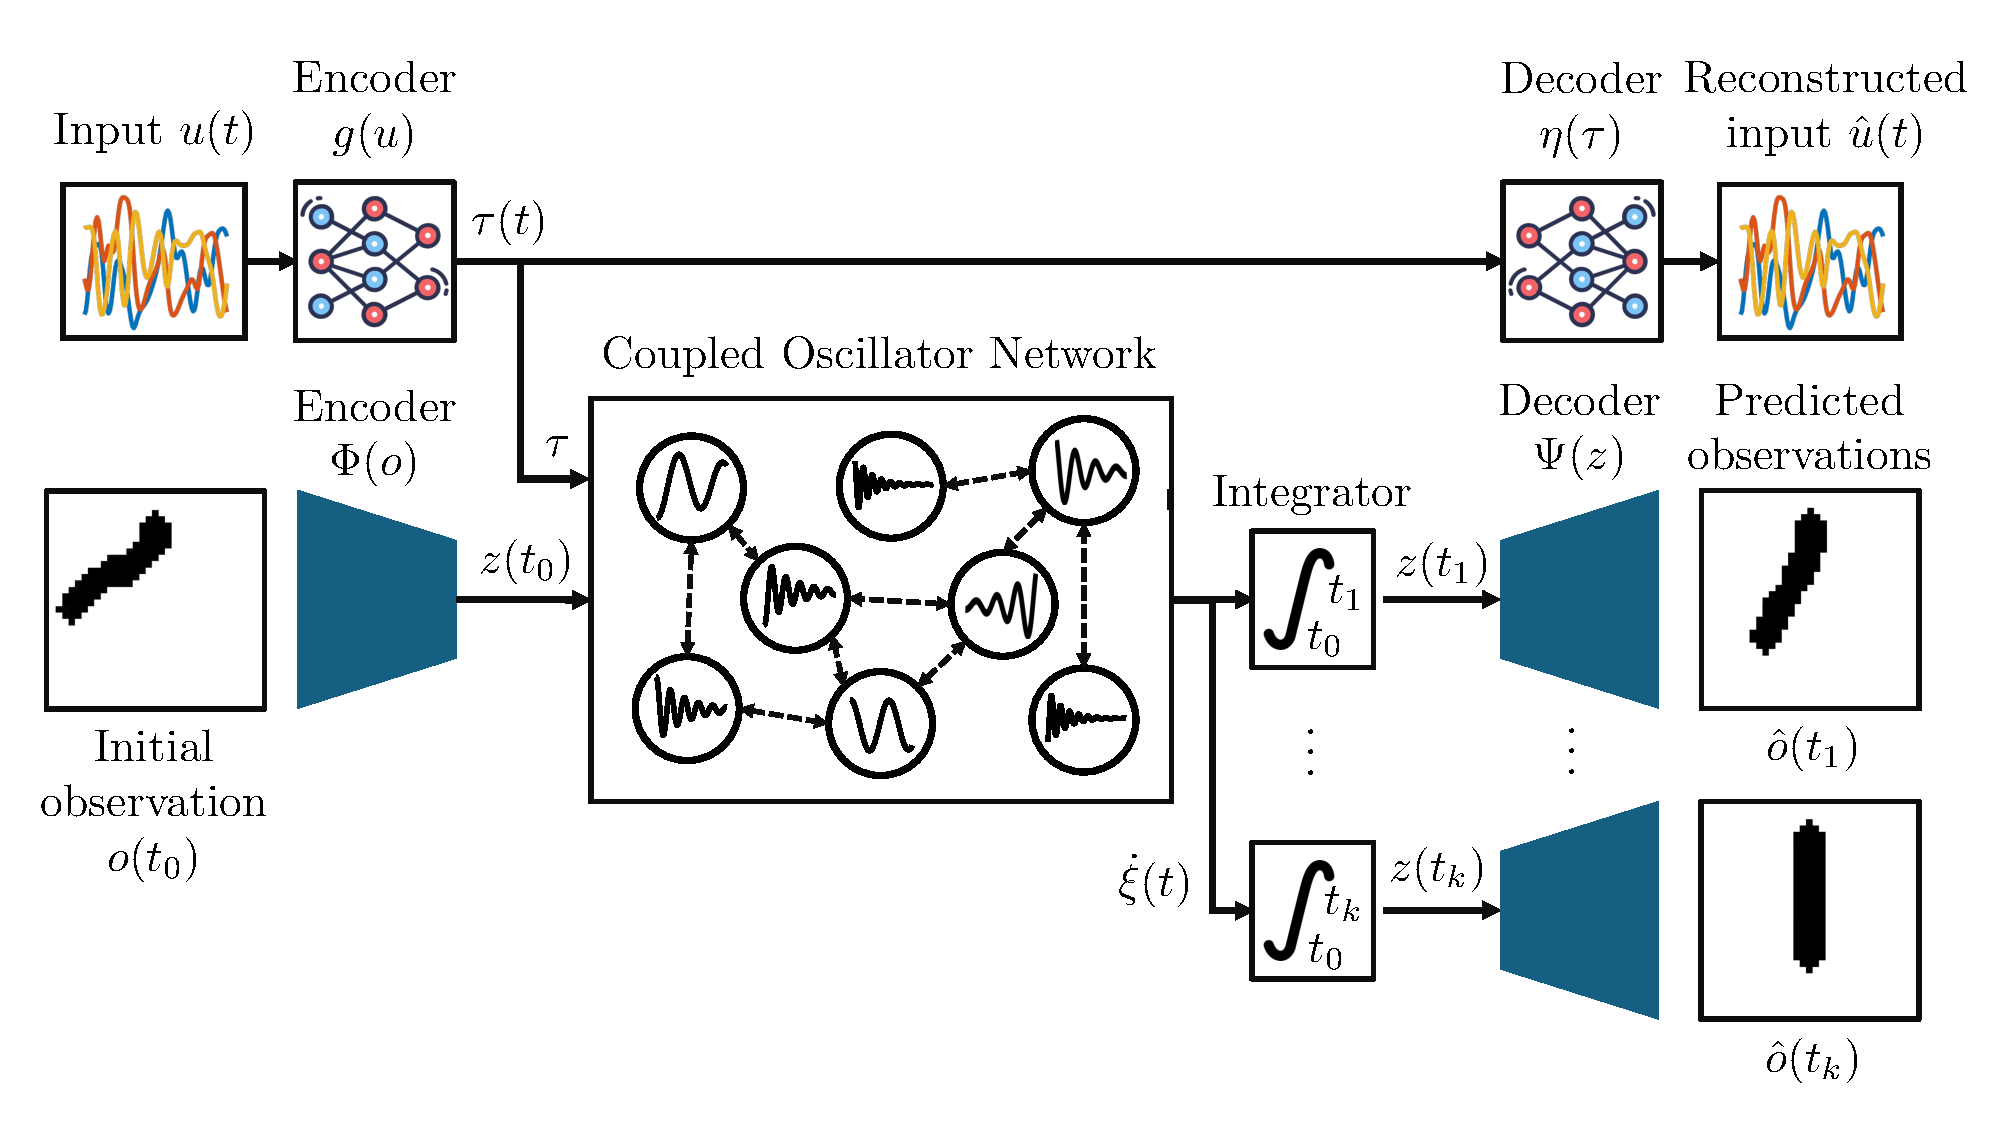
\includegraphics[width=1.0\linewidth]{con/figures/autoencoder/blockdiagram_autoencoder_v1_cropped.pdf}
    \caption{Exploiting \glspl{CON} for learning latent dynamics from pixels: We encode the initial observation $o(t_0)$ and the input $u(t)$ into latent space where we leverage the \gls{CON} to predict future latent states. Finally, we decode both the latent-space torques $\tau(t)$ and the predicted latent states $z(t)$.}
    \label{fig:con:blockdiagram_autoencoder}
\end{figure}

We assume to have access to observations in the form of images $o \in \mathbb{R}^{h_\mathrm{o} \times w_\mathrm{o} \times c_\mathrm{o}}$, where $c_\mathrm{o}$ denotes the number of channels. Please note that this could also be other high-dimensional observations such as LiDAR scans, point clouds, etc.
We now leverage an encoder-decoder architecture to map these high-dimensional observations into a compressed latent space: % parametrized by $z^\mathrm{T} & \dot{z}^\mathrm{T} \end{bmatrix}^\mathrm{T} \in \mathbb{R}^{2n_z}$.
The encoder $\Phi: \mathbb{R}^{h_\mathrm{o} \times w_\mathrm{o} \times c_\mathrm{o}} \to \mathbb{R}^{n_z} $ with $n_z \ll h_\mathrm{o} \,  w_\mathrm{o}$ identifies a low-dimensional latent representation $z \in \mathbb{R}^{n_z}$ of the images. The decoder $\Psi: \mathbb{R}^{n_z} \to \mathbb{R}^{h_\mathrm{o} \times w_\mathrm{o} \times c_\mathrm{o}}$ approximates the inverse operation by reconstructing an image $\hat{o} \in \mathbb{R}^{h_\mathrm{o} \times w_\mathrm{o} \times c_\mathrm{o}}$ based on the latent representation.
To promote the learning of a smooth and monotonic mapping into latent space, we specifically choose to implement the autoencoder here as a $\beta$-\gls{VAE}~\cite{kingma2014auto, higgins2017beta}.
Instead of just statically reconstructing the image $\hat{o}(t_k)$, we are interested in predicting future observations $\hat{o}(t_{k+l})$, where $l \in 1 \dots N$. For this, we train a \nth{2}-order dynamical model that is, when integrated, able to predict future latent representations $z(t_{k+l})$.
This requires us to define a latent state $\xi(t) = \begin{bmatrix}
    z^\mathrm{T}(t) & \dot{z}^\mathrm{T}(t)
\end{bmatrix}^\mathrm{T} \in \mathbb{R}^{2n_z}$ consisting of the latent representation and latent velocity $\dot{z}(t) \in \mathbb{R}^{n_z}$.

We now rely on \gls{CON} with $n = n_z$ oscillators to provide us with the latent state derivative $\dot{\xi}= f_\mathrm{w}(z(t), u(t))$, where we defined $\xi = y_\mathrm{w}$, and $z = x_\mathrm{w}$. To ensure stability, we make use of the Cholvesky decomposition to ensure that $M_\mathrm{w}, K_\mathrm{w}$ and $D_\mathrm{w}$ always remain positive definite (see Theorem~\ref{theorem:con:iss}).
It is important to note that we train the encoder, decoder, and dynamical model all jointly.
Please refer to Appendix~\ref{sec:apx-con:experimental_setup} for more implementation details.

% \begin{table}[ht]
%     \centering
%     \begin{scriptsize}
%     \begin{tabular}{c c c c c }
%          \toprule
%          \textbf{Model} & \textbf{RMSE PCC-NS-2} $\downarrow$ & \textbf{SSIM PCC-NS-2} $\uparrow$ & \textbf{RMSE CS} $\downarrow$ & \textbf{SSIM CS} $\uparrow$ \\
%          % \textbf{Model parameters} $\downarrow$ & \textbf{Training} $\frac{\mathbf{\text{steps}}}{\mathbf{\text{second}}}$ $\uparrow$ $\downarrow$
%          \midrule
%          RNN & $0.1373 \pm 0.0185$ & $0.9643 \pm 0.0077$ & $\mathbf{0.1011 \pm 0.0009}$ & $\mathbf{0.9776 \pm 0.0004}$ \\
%          GRU & $\mathbf{0.0951 \pm 0.0021}$ & $\mathbf{0.9814 \pm 0.0006}$ & $0.1125 \pm 0.0100$ & $0.9730 \pm 0.0040$\\
%          coRNN & $0.2504 \pm 0.0899$ & $0.8774 \pm 0.0857$ & $0.2537 \pm 0.0018$ & $0.8820 \pm 0.0024$\\
%          NODE & $0.1867 \pm 0.0561$ & $0.9279 \pm 0.0348$ & $0.2415 \pm 0.0021$ & $0.8946 \pm 0.0023$\\
%          MECH-NODE & $0.1035 \pm 0.0012$ & $0.9778 \pm 0.0004$ & $0.2494 \pm 0.0028$ & $0.8898 \pm 0.0016$\\
%          CON-S (our) & $0.0996 \pm 0.0012$ & $0.9792 \pm 0.0007$ & $0.1993 \pm 0.0646$ & $0.9218 \pm 0.0380$\\
%          CON-M (our) & $0.1008 \pm 0.0006$ & $0.9786 \pm 0.0003$ & $0.1063 \pm 0.0027$ & $0.9758 \pm 0.0011$\\
%          CFA-CON (our) & $0.1124 \pm 0.0025$ & $0.9734 \pm 0.0012$ & $0.1462 \pm 0.0211$ & $0.9730 \pm 0.0040$\\
%          \bottomrule
%     \end{tabular}
%     \end{scriptsize}
%     \caption{Benchmarking of \gls{CON} and \gls{CFA-CON} at learning latent dynamics for two datasets. The \emph{CS} dataset considers a continuum soft robot consisting of one segment with three constant planar strains. The \emph{PCC-NS-2} dataset contains \SI{2}{s} trajectories of a continuum soft robot made of two piecewise constant curvature segments. 
%     We choose the latent dimensions of the models as $n_z = 8$ and $n_z =12$ for the \emph{PCC-NS-2} and \emph{CS} datasets, respectively.
%     For the \glspl{RNN}, this corresponds to a hidden state dimension of $n_z=16$ and $n_z = 24$.
%     \emph{CON-S} and \emph{CON-M} are small and medium-sized versions of the \gls{CON} model, respectively. \emph{MECH-NODE} is a \gls{NODE} with prior knowledge about the mechanical structure of the system (i.e., $\frac{\mathrm{d}x}{\mathrm{d}t} = \dot{x}$).
%     We report the mean and standard deviation of the \gls{RMSE} and \gls{SSIM} metrics over three different random seeds.}
%     \label{tab:con:latent_dynamics_results}
% \end{table}
\begin{landscape}
\begin{table}
    \centering
    \begin{small}
    \setlength\tabcolsep{2pt}
    \begin{tabular}{c c c c c c c c}
         \toprule
         \textbf{Model} & \textbf{RMSE M-SP+F} $\downarrow$ & \textbf{RMSE S-P+F} $\downarrow$ & \textbf{RMSE D-P+F} $\downarrow$ & \textbf{RMSE CS} $\downarrow$ & \textbf{RMSE PCC-NS-2} $\downarrow$ & \textbf{RMSE PCC-NS-3} $\downarrow$ & \textbf{RMSE R-D} $\downarrow$ \\
         % \textbf{Model parameters} $\downarrow$ & \textbf{Training} $\frac{\mathbf{\text{steps}}}{\mathbf{\text{second}}}$ $\uparrow$ $\downarrow$
         \midrule
         RNN & $0.2739 \pm 0.0057$ & $0.2378 \pm 0.0352$ & $0.1694 \pm 0.0004$ & $\mathbf{0.1011 \pm 0.0009}$ & $0.1373 \pm 0.0185$ & $0.2232 \pm 0.0075$ & $0.3763 \pm 0.0374$\\
         GRU~\cite{cho2014learning} & $0.0267 \pm 0.0033$ & $0.1457 \pm 0.0078$ & $0.1329 \pm 0.0005$ & $0.1125 \pm 0.0100$ & $\mathbf{0.0951 \pm 0.0021}$ & $0.2148 \pm 0.0196$ & $0.3232 \pm 0.0368$\\
         coRNN~\cite{rusch2020coupled} & $\mathbf{0.0265 \pm 0.0002}$ & $0.1333 \pm 0.0044$ & $0.1324 \pm 0.0016$ & $0.2537 \pm 0.0018$ & $0.2504 \pm 0.0899$ & $0.2474 \pm 0.0018$ & $\mathbf{0.0741 \pm 0.0001}$\\
         NODE~\cite{chen2018neural} & $\mathbf{0.0264 \pm 0.0010}$ & $\mathbf{0.1260 \pm 0.0013}$ & $0.1324 \pm 0.0024$ & $0.2415 \pm 0.0021$ & $0.1867 \pm 0.0561$ & $0.3373 \pm 0.0565$ & $\mathbf{0.0738 \pm 0.0007}$\\
         MECH-NODE & $0.0328 \pm 0.0034$ & $0.1650 \pm 0.0205$ & $0.1710 \pm 0.0111$ & $0.2494 \pm 0.0028$ & $0.1035 \pm 0.0012$ & $0.1900 \pm 0.0024$ & N/A\\
         CON-S (our) & $0.0303 \pm 0.0053$ & $0.1303 \pm 0.0064$ & $0.1323 \pm 0.0018$ & $0.1993 \pm 0.0646$ & $0.0996 \pm 0.0012$ & $0.1792 \pm 0.0038$ & $0.1110 \pm 0.0160$\\
         CON-M (our) & $0.0303 \pm 0.0053$ & $0.1303 \pm 0.0064$ & $0.1323 \pm 0.0018$ & $0.1063 \pm 0.0027$ & $0.1008 \pm 0.0006$ & $\mathbf{0.1785 \pm 0.0023}$ & $0.1110 \pm 0.0160$\\
         CFA-CON (our) & $0.0313 \pm 0.0026$ & $0.1352 \pm 0.0073$ & $\mathbf{0.1307 \pm 0.0012}$ & $0.1462 \pm 0.0211$ & $0.1124 \pm 0.0025$ & $0.1803 \pm 0.0003$ & $0.1068 \pm 0.0059$\\
         \bottomrule
    \end{tabular}
    \end{small}
    \caption{Benchmarking of \gls{CON} and \gls{CFA-CON} at learning latent dynamics against baseline methods. 
    The first three datasets, based on ~\cite{botev2021priors}, contain samples of a mass-spring with friction (\emph{M-SP + F}), a single pendulum with friction (\emph{S-P + F}), and a double pendulum with friction (\emph{D-P + F}) (all without system inputs).
    The \emph{CS} dataset considers a continuum soft robot consisting of one segment with three constant planar strains. The \emph{PCC-NS-2} and \emph{PCC-NS-3} datasets contain trajectories of a continuum soft robot made of two and three piecewise constant curvature segments, respectively.
    We choose the latent dimensions of the models as $n_z = 4$, $n_z = 4$, and $n_z = 12$ for the \emph{M-SP + F}, \emph{S-P + F}, and \emph{D-P + F} datasets, and  $n_z = 8$, $n_z = 12$, and $n_z = 12$ for the \emph{PCC-NS-2}, \emph{PCC-NS-3}, and \emph{CS} soft robotic datasets.
    % For the \glspl{RNN}, this corresponds to a hidden state dimension of $n_z=16$ and $n_z = 24$.
    % \emph{CON-S} and \emph{CON-M} are small and medium-sized versions of the \gls{CON} model, respectively. \emph{MECH-NODE} is a \gls{NODE} with prior knowledge about the mechanical structure of the system (i.e., $\frac{\mathrm{d}x}{\mathrm{d}t} = \dot{x}$).
    We report the mean and standard deviation over three different random seeds.}
    \label{tab:con:latent_dynamics_results}
\end{table}

\begin{table}
    \centering
    \begin{small}
    \setlength\tabcolsep{2.5pt}
    \begin{tabular}{c|c|c|c|c|c|c|c|c|c}
        \toprule
        \textbf{Dataset} & $\mathbf{n_z}$ & \textbf{RNN} & \textbf{GRU}~\cite{cho2014learning} & \textbf{coRNN}~\cite{rusch2020coupled} & \textbf{NODE}~\cite{chen2018neural} & \textbf{MECH-NODE} & \textbf{CON-S (our)} & \textbf{CON-M (our)} & \textbf{CFA-CON (our)}\\
        \midrule
        M-SP+F~\cite{botev2021priors} & $4$ & $88$ & $248$ & $40$ & $3368$ & $3244$ & $\mathbf{34}$ & $\mathbf{34}$ & $\mathbf{34}$\\
        S-P+F~\cite{botev2021priors} & $4$ & $88$ & $248$ & $40$ & $3368$ & $3244$ & $\mathbf{34}$ & $\mathbf{34}$ & $\mathbf{34}$\\
        D-P+F~\cite{botev2021priors} & $12$ & $672$ & $1968$ & $348$ & $4404$ & $4032$ & $\mathbf{246}$ & $\mathbf{246}$ & $\mathbf{246}$\\
        CS & $12$ & $696$ & $2040$ & $\mathbf{336}$ & $4374$ & $4002$ & $1386$ & $8568$ & $8568$\\
        PCC-NS-2 & $8$ & $320$ & $928$ & $\mathbf{152}$ & $3856$ & $3062$ & $676$ & $7048$ & $7048$\\
        PCC-NS-3 & $12$ & $696$ & $2040$ & $\mathbf{336}$ & $4374$ & $4002$ & $1386$ & $8568$ & $8568$\\
        R-D~\cite{champion2019data} & $4$ & $\mathbf{20}$ & $52$ & $\mathbf{20}$ & $3064$ & - & $24$ & $24$ & $24$\\
        \bottomrule
    \end{tabular}
    \end{small}
    \caption{Number of trainable parameters for the each latent dynamic models depending on the respective dataset: mass-spring with friction (\emph{M-SP+F}), single pendulum with friction (\emph{S-P+F}), double pendulum with friction (\emph{D-P+F}), a constant strain soft robot (\emph{CS}), a piecewise constant curvature with two segments (\emph{PCC-NS-2}, a piecewise constant curvature soft robot with three segments (\emph{PCC-NS-3}, and reaction-diffusion (\emph{R-D}).}
    \label{tab:con:latent_dynamics_number_of_parameters}
\end{table}
\end{landscape}

\begin{figure}[ht]
    \centering
    \subfigure[RMSE vs. latent dimension $n_z$]{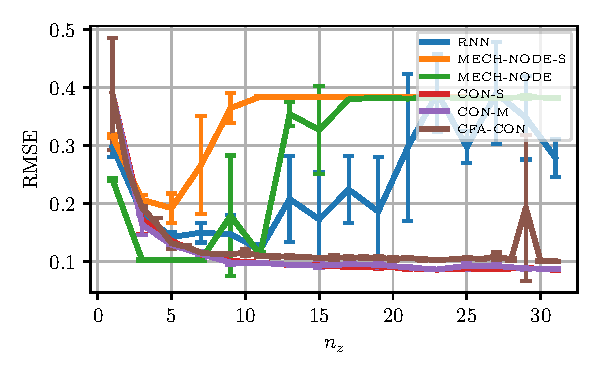
\includegraphics[width=0.45\textwidth, trim={5, 5, 5, 5}]{con/figures/results/latent_dynamics/pcc_ns-2/sweep_rmse_rec_dynamic_vs_n_z.pdf}}
    \subfigure[RMSE vs. model parameters]{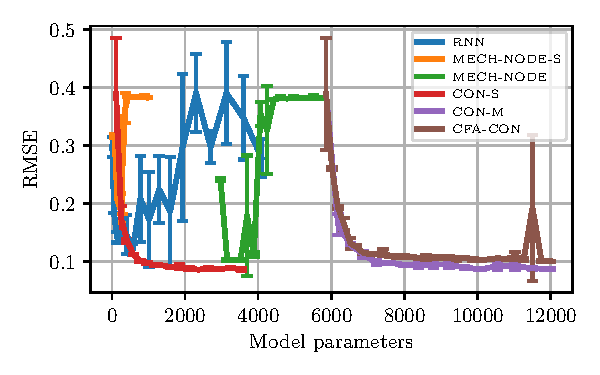
\includegraphics[width=0.45\textwidth, trim={5, 5, 5, 5}]{con/figures/results/latent_dynamics/pcc_ns-2/sweep_rmse_rec_dynamic_vs_num_trainable_params.pdf}}
    \caption{Evaluation of prediction performance of the various models vs. the dimension of their latent representation $n_z$ and the number of trainable parameters of the dynamics model, respectively, on the \emph{PCC-NS-2} dataset. All hyperparameters are tuned for each model separately for $n_z=8$. The error bar denotes the standard deviation across three random seeds.} \label{fig:con:latent_dynamics_sweep_pcc_ns-2}
\end{figure}

\subsection{Training} 
It is important to remember that because we are using a $\beta$-\gls{VAE}~\cite{kingma2014auto, higgins2017beta}, the image encoding becomes stochastic, and the encoder neural network actually outputs $\mu_z(o), 2 \, \log(\sigma_z)(o) \in \mathbb{R}^{n_z}$. After executing the reparametrization trick as $z(t_k) \sim \mathcal{N}(\mu_z(t_k), \sigma_z^2(t_k))$, we formulate the loss function, evaluated on each trajectory consisting of $N$ time-steps, as
\begin{equation}\label{eq:training_loss}
\begin{split}
    \mathcal{L} =& \: \sum_{k=0}^{N} \left ( \underbrace{\frac{\mathrm{MSE}(o(t_k), \Psi(z(t_k)))}{N+1}}_{\text{Static image reconstruction loss}} + \beta \underbrace{\frac{\mathcal{D}_\mathrm{KL} \left ( (\mu_z(t_k), \sigma_z(t_k) \right )}{N+1}}_{\text{Kullback–Leibler divergence}} \right )\\
    &\: + \sum_{k=1}^{N} \left ( \lambda_{\vec{o}} \underbrace{ \frac{\mathrm{MSE}(o(t_k), \Psi(\hat{z}(t_k)))}{N}}_{\text{Dynamic image reconstruction loss}} + \lambda_{\mathrm{z}} \underbrace{\frac{\mathrm{MSE}(z(t_k), \hat{z}(t_k))}{N}}_{\text{Latent dynamics consistency loss}} \right ),
\end{split}
\end{equation}
where $\hat{z}(t_k)$ is predicted by $\hat{\xi}(t_k)  = \int_{t=t_0}^{t_k} f_\xi(\xi(t'), u(t')) \: \mathrm{d}t'$, and $\xi(t_0) = \begin{bmatrix}
    z^\mathrm{T}(t_0) & \dot{z}^\mathrm{T}(t_0)
\end{bmatrix}^\mathrm{T}$. Here, $z(t_0)$ is given by the encoder, and $\dot{z}(t_0)$ is approximated using finite differences in image-space. $\beta, \lambda_{\vec{o}}, \lambda_\mathrm{z} \in \mathbb{R}$ are loss weights.

\subsubsection{Estimation of the initial latent velocity}\label{sub:con:initial_latent_velocity_estimation}
For \nth{2}-order systems and when integrating the evolution of the latent state $\xi(t) = \begin{bmatrix}
    z^\mathrm{T}(t) & \dot{z}^\mathrm{T}(t)
\end{bmatrix}^\mathrm{T}$ in time, we need to have access to an initial latent velocity $\dot{z}(t_0)$ such that we can roll out the latent state $\xi(t)$ in time.
A naive approach to estimating such an initial latent velocity would be to encode multiple (at least two) images of the system at the start of the trajectory into latent space and then perform numerical differentiation (e.g., finite differences) in latent space. However, we found the resulting $\dot{z}(t_k)$ to be relatively noisy and susceptible to small encoding errors.
Instead, we propose to perform numerical differentiation in image space and then map this velocity into latent space using the encoder's Jacobian. First, we estimate the image-space velocity at $t_k$ using finite differences: $\dot{o}(t_k) \approx \frac{o(t_{k+1}) - o(t_{k-1})}{t_{k+1} - t_{k-1}}$. The latent velocity is then estimated as $\dot{z}(t_k) = \frac{\partial \Phi}{\partial o} (o(t_k)) \, \dot{o}(t_k)$, where $\frac{\partial \Phi}{\partial o}$ is obtained with forward-mode automatic differentiation.

\subsection{Models} 
We train the \gls{CON} with the input-to-forcing mapping $g(u) = B(u) \, u$, where $B(u)$ is parametrized by a \gls{MLP} with a hyperbolic tangent activation function applied in between layers. We report results for two variants of the \gls{CON} model: for the medium-sized \emph{CON-M} and small-sized \emph{CON-S}, the \gls{MLP} consists of five and two layers with a hidden dimension of $30$ and $12$, respectively. The model \gls{CFA-CON} uses the same architecture as \emph{CON-M}. We compare % the performance of our proposed models 
against several popular latent space model architectures:
The \gls{NODE} model uses a \gls{MLP} with an hyperbolic activation functions and predicts $\dot{\xi}(t) = f_\mathrm{NODE}(\xi(t), u(t))$. To make the comparison fair, we parametrize the NODE's \gls{MLP} in the same fashion as for \emph{CON-M}. The \emph{MECH-NODE} integrates prior knowledge towards learning \nth{2}-order mechanical \glspl{ODE} and, therefore, predicts $\ddot{z}(t) = f_\mathrm{MECH-NODE}(\xi(t), u(t))$. 
Furthermore, we consider multiple autoregressive models: \gls{RNN}, \gls{GRU}, and \gls{coRNN} and let them parameterize the following transition function: $\xi(t_{k+1}) = f_\mathrm{ar}(\xi(t_k), u(t_k))$
As common in the relevant literature~\cite{botev2021priors}, we allow the autoregressive models to perform multiple time step transitions before predicting the next sample.
For the autoencoder, we use a vanilla \gls{CNN}. More details can be found in Appendix~\ref{sec:apx-con:experimental_setup}.

\subsection{Datasets} 
We consider in total seven datasets that are based on simulations of unactuated mechanical systems, actuated continuum soft robots, and the reaction-diffusion dynamics. The first three, mechanical dataset are based on the work of Botev et al.~\cite{botev2021priors} and contain video sequences of a mass-spring system with friction (\emph{M-SP+F}), a single pendulum with friction (\emph{S-P+F}), and a double pendulum with friction (\emph{D-P+F}).
Continuum soft robots have theoretically infinite \gls{DOF}, evolve with highly nonlinear and often time-dependent dynamical behaviors, and are notoriously difficult to model from first principles~\cite{armanini2023soft}. For that reason, it is a very interesting proposition if we could learn latent-space dynamical models directly from video~\cite{thuruthel2023multi} and later leverage them for control~\cite{almanzor2023static}. 
Therefore, we generate three datasets based on the \gls{PCS} soft robot model. \emph{CS} considers one segment with constant strain and is modeled using three configuration variables. \emph{PCC-NS-2} and \emph{PCC-NS-3} only consider bending deformations and contain soft robots with two and three segments, respectively. 
As all previous examples exampled \glspl{ODE}, we strive to test the proposed approach also on a system that is governed by \glspl{PDE}. Specifically, we consider the Reaction-diffusion (\emph{R-D}) dataset as included in the SINDy Autoencoder paper~\cite{champion2019data}.
For all datasets, we generate images of size $32 \times 32 \mathrm{px}$ and subsequently normalize the pixels to the interval $[-1, 1]$. 
% We tune all hyperparameters for each model and dataset separately using Optuna~\cite{akiba2019optuna}.

\subsubsection{Unactuated mechanical datasets}
We consider multiple mechanical datasets based on a standard implementation included in the \emph{Toy Physics} category of the \emph{NeurIPS 2021 Track on Datasets and Benchmarks} publication by Botev et al.~\cite{botev2021priors}:  mass-spring with friction (M-SP+F), a single pendulum with friction (S-P+F), and a double pendulum with friction (D-P+F).
All datasets contain $5000$ system trajectories in the training set and $1000$ trajectories each in the validation and test set.
Each trajectory is generated by first randomly initializing the system, then rolling it out for $\SI{3}{s}$ using an Euler integrator with a time step size of $\SI{5}{ms}$. Samples are recorded at a rate of \SI{20}{Hz}  (i.e., a time step of \SI{0.05}{s}). As a result, each trajectory contains $60$ images of the system's state.
As all of these datasets are unactuated, we can deactivate the input-to-forcing mapping component from all models (e.g., set $g(u) = 0$ for the \gls{CON} model).

The \emph{M-SP+F} dataset contains motion samples of a damped harmonic oscillator with a mass of $\SI{0.5}{kg}$, a spring stiffness of \SI{2}{N \per m}, and a damping coefficient of \SI{0.05}{Ns \per m}. For each trajectory, the initial condition of the mass-spring is randomly sampled by combining a random $\mathrm{sign}(q)$ with a uniformly sampled $|q| \sim \mathcal{U}(\SI{0.1}{m}, \SI{1}{m})$. The position of the mass is rendered with a filled circle in a grayscale image.

The \emph{SP+F} and \emph{DP+F} datasets include the evolutions of a single-link pendulum and double-link pendulum, respectively, with a mass of \SI{0.5}{kg} attached to the end of each link, which has a length of \SI{1}{m}. The dataset considers a gravitational acceleration of $\SI{3}{m \per s^2}$. A rotational damper with coefficient \SI{0.05}{Nms \per rad} provides the friction. 
Similarly to the \emph{M-SP+F} dataset, both the sign and the absolute value of the initial configuration are randomly sampled, where $|q(0)| \sim \mathcal{U}(\SI{1.3}{rad}, \SI{2.3}{rad})$.
The position of each mass is rendered with a filled circle. For the single-link pendulum, this is done in grayscale, and for the double pendulum, each mass is rendered with a different color (i.e., blue and red).

\subsubsection{Actuated continuum soft robot datasets}\label{ssub:con:soft_robot_dataset}
The shape of slender and deformable rods can be approximated by considering the deformations along the 1D curve of the backbone~\cite{gazzola2018forward}. While this curve is still infinite-dimensional, it is possible to discretize the backbone into (many) segments with piecewise constant strain~\cite{renda2016discrete, gazzola2018forward}.
Accordingly, we describe the kinematics of a planar continuum soft robot consisting of $n_\mathrm{b}$ segments with the \gls{PCS} model~\cite{renda2016discrete}. We assume each segment has a length of \SI{100}{mm} and a diameter of \SI{20}{mm}.
The \gls{PCS} model assumes each segment to have constant strain. In the planar case, this means that the shape of the $i$th segment can be parametrized by $\xi_i = \begin{bmatrix}
    \kappa_{\mathrm{be},i} & \sigma_{\mathrm{sh},i} & \sigma_{\mathrm{ax},i}
\end{bmatrix}^\mathrm{T} \in \mathbb{R}^{3}$ where $\kappa_{\mathrm{be},i}$ is the bending strain (i.e., the curvature) in the unit \si{rad \per \meter}, $\sigma_{\mathrm{sh},i}$ is the shear strain  (dimensionless), and $\sigma_{\mathrm{ax},i}$ is the axial elongation strain (dimensionless).
The robot's configuration is then defined as $q = \begin{bmatrix}
    \xi_1^\mathrm{T} & \cdots & \xi_i^\mathrm{T} & \cdots & \xi_{n_\mathrm{b}}^\mathrm{T}
\end{bmatrix}^\mathrm{T}$.
In the case of \gls{PCC}, only the bending strain is active as shear strains and axial strains are neglected, and the configuration is now $q \in \mathbb{R}^{n_\mathrm{b}}$.
The \gls{PCS} model generates \gls{EOM} in the form of~\cite{della2023model}
\begin{equation}
    B(q) \, \ddot{q} + C(q,\dot{q}) \, \dot{q} + G(q) + K_\mathrm{q} \, q + D_\mathrm{q} \, \dot{q} = u(t),
\end{equation}
where $B(q) \succ 0$ and $C(q,\dot{q})$ are the inertia and Corioli matrices, respectively. $G(q)$ collects the gravitational forces, $K_\mathrm{q} \succ 0$ is the stiffness matrix, and $D_\mathrm{q} \succ 0$ contains the damping coefficients. 
$u(t) \in \mathbb{R}^{n_\mathrm{b}}$ is an external force acting on the generalized coordinates, and now $m = n_\mathrm{b}$.

% \begin{figure}
%     \centering
%     \includegraphics[width=0.5\columnwidth]{figures/soft_robot/katzschmann_planar_soft_robot.png}
%     \caption{A planar soft robot, consisting of six segments, that deforms with piecewise constant curvature. The behavior of the simulated robots included in datasets \emph{PCC-NS-2} and \emph{PCC-NS-3} resembles this pneumatically actuated robot. The source of the image is (Della Santina et al., 2020)~\cite{della2020model}.}
%     \label{fig:enter-label}
% \end{figure}

We derive the corresponding dynamics for a continuum soft robot of material density $\SI{600}{kg \per \meter^3}$, elastic modulus of \SI{20000}{Pa}, shear modulus of \SI{10000}{Pa}, and damping coefficients of \SI{0.00001}{Nm^2s} for bending strains, \SI{0.01}{Ns} for shear strains, and \SI{0.01}{Ns} for axial strains, respectively.
Gravity is pointing downwards.
The implementation of the dynamics in JAX~\cite{jax2018github} is based on the \emph{JSRM} library~\cite{stolzle2024experimental, stolzle2024guiding}, and we simulate the robot using a constant integration time step of \SI{0.1}{ms}.
We render grayscale images of the robot with a size of $32 \times 32 \mathrm{px}$ at a rate of \SI{50}{Hz} using OpenCV~\cite{opencv_library}. 
We generate $10000$ trajectories, each of duration \SI{2.0}{s} and a sampling time-step of $\SI{0.02}{s}$. We use \SI{60}{\percent} training, \SI{20}{\percent} validation, and \SI{20}{\percent} test split.
For each trajectory, we randomly sample a constant actuation/input $u \sim \mathcal{U}(-u_\mathrm{max}, u_\mathrm{max})$. We choose the maximum actuation magnitude to be equal to the sum of the contribution of the potential forces (i.e., elastic and gravitational forces): $u_\mathrm{max} = G(q_\mathrm{max}) + K \, q_\mathrm{max}$ with $q_{\mathrm{max},i} = \begin{bmatrix}
    5 \, \pi~\si{rad \per m}, 0.2, 0.2
\end{bmatrix}^\mathrm{T}$.

We generate three datasets based on this continuum soft robot model: in the \emph{CS} dataset, we consider one segment with all three planar strains active (i.e., bending, shear, and elongation). This results in three \gls{DOF} and six-state variables in the dynamical model. In the case of the \emph{PCC-NS-2} and \emph{PCC-NS-3} datasets, we base the dataset on a simulated system consisting of two planar bending segments, respectively. Each segment is parametrized using \gls{CC}~\cite{webster2010design, rosi2022sensing}, which results in two configuration variables and a state dimension of four.

\subsubsection{Unactuated PDE reaction-diffusion dataset}\label{ssub:con:reaction_diffusion_dataset}
 We consider the \nth{1}-order Reaction-diffusion (\emph{R-D}) \gls{PDE} on which (Champion et al, 2019)~\cite{champion2019data} evaluated their SINDy Autoencoder on. The \gls{PDE} of the high-dimensional lambda-omega reaction-diffusion system is defined as
\begin{equation}
\begin{split}
    \frac{\partial u}{\partial t} =& \: \left ( 1 - (u^2 + v^2) \right ) u + \beta \, (u^2 + v^2) \, v + d_1 \left ( \frac{\partial^2 u}{\partial q_1^2} + \frac{\partial^2 u}{\partial q_2^2} \right ),\\
    \frac{\partial v}{\partial t} =& \: -\beta (u^2 + v^2) \, u + (1 - (u^2 + v^2)) \, v + d_2 \left ( \frac{\partial^2 v}{\partial q_1^2} + \frac{\partial^2 v}{\partial q_2^2} \right ),
\end{split}
\end{equation}
where $u(t,q): \mathbb{R} \times \mathbb{R}^2 \to \mathbb{R}$ and $v(t,q): \mathbb{R} \times \mathbb{R}^2 \to \mathbb{R}$ are time-dependent two vector fields defined over the spatial domain $q \in \mathbb{R}^2$.
We choose the same system parameters and initial condition as Champion et al.~\cite{champion2019data}: $d_1, d_2 = 0.1$, and $\beta = 1$ and 
\begin{equation}
\begin{split}
    u(0,q) = \tanh \left ( \sqrt{q_1^2 + q_2^2} \, \cos \left ( \angle (q_1 + i q_2) - \sqrt{q_1^2 + q_2^2} \right ) \right ),\\
    v(0,q) = \tanh \left ( \sqrt{q_1^2 + q_2^2} \, \sin \left ( \angle (q_1 + i q_2) - \sqrt{q_1^2 + q_2^2} \right ) \right ).
\end{split}
\end{equation}

After discretizing the spatial domain into $32$ points along each dimension, we solve the \gls{PDE} with a MATLAB ODE45 solver the solution of $u(t,q)$ and $v(t,q)$ at each time step and grid point.
Subsequently, the solution is multiplied with a Gaussian centered at the origin~\cite{champion2019data}
\begin{equation}
\begin{split}
    \bar{u}(t,q) =& \: \exp(-0.01 \, (q_1^2 + q_2^2)) \, \bar{u}(t,q),\\
    \bar{v}(t,q) =& \: \exp(-0.01 \, (q_1^2 + q_2^2)) \, \bar{v}(t,q).
\end{split}
\end{equation}
We integrate the system from the specified initial condition for \SI{500}{s} and store samples at a time step of \SI{0.05}{s}. We divide the entire sequence into $99$ subsequences each containing $101$ samples. We train the models to predict these subsequences that have a horizon of $\SI{5.0}{s}$ each.

We stack the solution of $\bar{u}(t, q)$ and $\bar{v}(t,q)$ contained in the two grids $o_\mathrm{u}(t), o_\mathrm{v}(t) \in \mathbb{R}^{32 \times 32}$, respectively, to gather the images $o(t) \in \mathbb{R}^{32 \times 32 \times 2}$ containing two channels.
A sample sequence of the generated images is presented in Fig.~\ref{fig:con:latent_dynamics:sequence_of_stills:r_d:rollout2}.
We use \SI{60}{\percent} of the subsequences (i.e., $59$) as our training set, and employ \SI{20}{\percent} (i.e., $19$) for the validation and test sets, respectively. 

\subsection{Results}

\subsubsection{Results for unactuated mechanical datasets}
The results in Tab.~\ref{tab:con:latent_dynamics_results} show that the \emph{NODE} model slightly outperforms the \emph{CON} network on the \emph{M-SP+F} and \emph{S-P+F} datasets. However, as the datasets do not consider system inputs, we can remove the input mapping from all models (e.g., \emph{RNN}, \emph{GRU}, \emph{coRNN}, \emph{CON}, and \emph{CFA-CON}). With that adjustment, the \emph{CON} network has the fewest parameters among all models, particularly two orders of magnitude less than the NODE model. Therefore, we find it very impressive that the CON network is roughly on par with the NODE model. For the \emph{D-P+F} dataset, we can conclude that the \emph{CFA-CON} model offers the best performance across all methods. Finally, most of the time, the \emph{CON} \& \emph{CFA-CON} networks outperform the other baseline methods that have more trainable parameters.
Sequences of stills of the rollout of the \gls{CON} model trained on the \emph{M-SP+F}, and \emph{D-P+F} datasets are presented in Figs.~\ref{fig:con:latent_dynamics:sequence_of_stills:m-sp+f:rollout3} and \ref{fig:con:latent_dynamics:sequence_of_stills:d-p+f:rollout7}.

\subsubsection{Results for actuated continuum soft robot datasets} 
The results in Tab.~\ref{tab:con:latent_dynamics_results} show that \emph{CON-M} matches the performance of the state-of-the-art methods across all experiments. In the case of \emph{PCC-NS-3}, \emph{CON-M} even decreases the \gls{RMSE} error by \SI{6}{\percent} w.r.t. the closest baseline method (MECH-NODE).
Impressively, the performance is not reduced (but instead often even improved) compared to other models that offer a much larger design space for learning the dynamics (e.g. \gls{NODE}).
Furthermore, \emph{CON-S} and \emph{CFA-CON} often only exhibit slightly lower performance than \emph{CON-M}, even though they have significantly fewer parameters and consider an approximated solution, respectively.
Supplementary results (e.g., more evaluation metrics) can be found in Appendix~\ref{sec:apx-con:latent_dynamics_results}. Sequences of stills for the \gls{CON} model trained on the \emph{PCC-NS-3} dataset are provided in Fig.~\ref{fig:con:latent_dynamics:sequence_of_stills:pcc_ns-3:rollout4}.

We also conduct on the \emph{PCC-NS-2} dataset an analysis concerning the effect of the latent dimension on the performance (see Fig.~\ref{fig:con:latent_dynamics_sweep_pcc_ns-2}). For this experiment, all hyperparameters were tuned for $n_z=8$, and we observe that the \gls{CON} models have a much-improved consistency and smaller variance w.r.t. the baseline methods when the latent dimensionality is increased.

\subsubsection{Results for reaction-diffusion dataset}
To address the unactuated nature of the \emph{R-D} dataset, we remove, analog to the \emph{M-SP+F}, \emph{S-P+F}, and \emph{D-P+F} datasets, the input-to-state mapping parameters of the dynamical models (e.g., the $B(u)$ and $E(\tau)$ \glspl{MLP} for the \gls{CON} models).
Furthermore, the \gls{PDE} describing the system dynamics is of \nth{1}-order. Therefore, we leverage the \nth{1}-order versions of the latent dynamics, in particular for the \emph{coRNN}, \emph{CON}, \emph{CFA-CON} models, as specified in Apx.~\ref{sub:apx-con:1st_order_latent_dynamics}.
We report the \gls{RMSE} of the test set evaluations in Tab.~\ref{tab:con:latent_dynamics_results}. Furthermore, we also present a sequence of stills of the rollout of a trained latent dynamics \gls{CON} model in Fig.~\ref{fig:con:latent_dynamics:sequence_of_stills:r_d:rollout2}.
We find it impressive that \gls{CON} with its strong stability guarantees can accurately model the dynamics of a high-dimensional \gls{PDE} system.
Still, these initial results show that, for a comparable number of model parameters, the \gls{coRNN} model exhibits a \SI{32}{\percent} better performance than the \gls{CON} model. Therefore, in particular as \gls{coRNN} and \gls{CON} are both oscillatory networks, it would be interesting to analze in future work which characteristic gives \gls{coRNN} the most performance benefits compared to \gls{CON} on this \gls{PDE} datasets.

\begin{figure}[hb]
    \centering
    \subfigure{
\includegraphics[width=0.160\columnwidth]{con/figures/results/latent_dynamics/m-sp+f/sequence_of_stills/rollout_3_target_0.00.png}}
    \subfigure{
\includegraphics[width=0.160\columnwidth]{con/figures/results/latent_dynamics/m-sp+f/sequence_of_stills/rollout_3_target_0.55.png}}
    \subfigure{
\includegraphics[width=0.160\columnwidth]{con/figures/results/latent_dynamics/m-sp+f/sequence_of_stills/rollout_3_target_1.10.png}}
    \subfigure{
\includegraphics[width=0.160\columnwidth]{con/figures/results/latent_dynamics/m-sp+f/sequence_of_stills/rollout_3_target_1.65.png}}
    \subfigure{
\includegraphics[width=0.160\columnwidth]{con/figures/results/latent_dynamics/m-sp+f/sequence_of_stills/rollout_3_target_2.20.png}}
    \subfigure{
\includegraphics[width=0.160\columnwidth]{con/figures/results/latent_dynamics/m-sp+f/sequence_of_stills/rollout_3_target_2.75.png}}
    \\
    \setcounter{subfigure}{0}
    \subfigure[t=\SI{0.0}{s}]{
\includegraphics[width=0.160\columnwidth]{con/figures/results/latent_dynamics/m-sp+f/sequence_of_stills/rollout_3_pred_0.00.png}}
    \subfigure[t=\SI{0.55}{s}]{
\includegraphics[width=0.160\columnwidth]{con/figures/results/latent_dynamics/m-sp+f/sequence_of_stills/rollout_3_pred_0.55.png}}
    \subfigure[t=\SI{1.10}{s}]{
\includegraphics[width=0.160\columnwidth]{con/figures/results/latent_dynamics/m-sp+f/sequence_of_stills/rollout_3_pred_1.10.png}}
    \subfigure[t=\SI{1.65}{s}]{
\includegraphics[width=0.160\columnwidth]{con/figures/results/latent_dynamics/m-sp+f/sequence_of_stills/rollout_3_pred_1.65.png}}
    \subfigure[t=\SI{2.20}{s}]{
\includegraphics[width=0.160\columnwidth]{con/figures/results/latent_dynamics/m-sp+f/sequence_of_stills/rollout_3_pred_2.20.png}}
    \subfigure[t=\SI{2.75}{s}]{
\includegraphics[width=0.160\columnwidth]{con/figures/results/latent_dynamics/m-sp+f/sequence_of_stills/rollout_3_pred_2.75.png}}
    \caption{Prediction sequence of a \gls{CON} model with latent dimension $n_z=4$ trained on the damped harmonic oscillator (\emph{M-SP+F}) dataset~\cite{botev2021priors}. 
    \textbf{Top row:} Ground-truth evolution of the system. \textbf{Bottom row:} Predictions of the \emph{CON} model. \newline
    The prediction model is given three images centered around $t=0$ for encoding the initial latent $z(0)$ and estimation of the initial latent velocity $\dot{z}(0)$. Subsequently, we roll out the autonomous network dynamics (i.e., unforced) and compare the decoded predictions with the ground-truth evolution of the system.  
    }\label{fig:con:latent_dynamics:sequence_of_stills:m-sp+f:rollout3}
\end{figure}

\begin{figure}[hb]
    \centering
    \subfigure{
\includegraphics[width=0.160\columnwidth]{con/figures/results/latent_dynamics/d-p+f/sequence_of_stills/rollout_7_target_0.00.png}}
    \subfigure{
\includegraphics[width=0.160\columnwidth]{con/figures/results/latent_dynamics/d-p+f/sequence_of_stills/rollout_7_target_0.55.png}}
    \subfigure{
\includegraphics[width=0.160\columnwidth]{con/figures/results/latent_dynamics/d-p+f/sequence_of_stills/rollout_7_target_1.10.png}}
    \subfigure{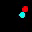
\includegraphics[width=0.160\columnwidth]{con/figures/results/latent_dynamics/d-p+f/sequence_of_stills/rollout_7_target_1.65.png}}
    \subfigure{
\includegraphics[width=0.160\columnwidth]{con/figures/results/latent_dynamics/d-p+f/sequence_of_stills/rollout_7_target_2.20.png}}
    \subfigure{
\includegraphics[width=0.160\columnwidth]{con/figures/results/latent_dynamics/d-p+f/sequence_of_stills/rollout_7_target_2.75.png}}
    \\
    \setcounter{subfigure}{0}
    \subfigure[t=\SI{0.0}{s}]{
\includegraphics[width=0.160\columnwidth]{con/figures/results/latent_dynamics/d-p+f/sequence_of_stills/rollout_7_pred_0.00.png}}
    \subfigure[t=\SI{0.55}{s}]{
\includegraphics[width=0.160\columnwidth]{con/figures/results/latent_dynamics/d-p+f/sequence_of_stills/rollout_7_pred_0.55.png}}
    \subfigure[t=\SI{1.10}{s}]{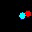
\includegraphics[width=0.160\columnwidth]{con/figures/results/latent_dynamics/d-p+f/sequence_of_stills/rollout_7_pred_1.10.png}}
    \subfigure[t=\SI{1.65}{s}]{
\includegraphics[width=0.160\columnwidth]{con/figures/results/latent_dynamics/d-p+f/sequence_of_stills/rollout_7_pred_1.65.png}}
    \subfigure[t=\SI{2.20}{s}]{
\includegraphics[width=0.160\columnwidth]{con/figures/results/latent_dynamics/d-p+f/sequence_of_stills/rollout_7_pred_2.20.png}}
    \subfigure[t=\SI{2.75}{s}]{
\includegraphics[width=0.160\columnwidth]{con/figures/results/latent_dynamics/d-p+f/sequence_of_stills/rollout_7_pred_2.75.png}}
    \caption{Prediction sequence of a \gls{CON} model with latent dimension $n_z=12$ trained on the double pendulum with friction (\emph{D-P+F}) dataset~\cite{botev2021priors}. 
    \textbf{Top row:} ground-truth evolution of the system. \textbf{Bottom row:} predictions of the \emph{CON} model. \newline
    The prediction model is given three images centered around $t=0$ for encoding the initial latent $z(0)$ and estimation of the initial latent velocity $\dot{z}(0)$. Subsequently, we roll out the autonomous network dynamics (i.e., unforced) and compare the decoded predictions with the ground-truth evolution of the system.  
    }\label{fig:con:latent_dynamics:sequence_of_stills:d-p+f:rollout7}
\end{figure}

\begin{figure}[hb]
    \centering
    \subfigure{
\includegraphics[width=0.160\columnwidth]{con/figures/results/latent_dynamics/pcc_ns-3/sequence_of_stills/rollout_4_target_0.00.png}}
    \subfigure{
\includegraphics[width=0.160\columnwidth]{con/figures/results/latent_dynamics/pcc_ns-3/sequence_of_stills/rollout_4_target_0.36.png}}
    \subfigure{
\includegraphics[width=0.160\columnwidth]{con/figures/results/latent_dynamics/pcc_ns-3/sequence_of_stills/rollout_4_target_0.72.png}}
    \subfigure{
\includegraphics[width=0.160\columnwidth]{con/figures/results/latent_dynamics/pcc_ns-3/sequence_of_stills/rollout_4_target_1.08.png}}
    \subfigure{
\includegraphics[width=0.160\columnwidth]{con/figures/results/latent_dynamics/pcc_ns-3/sequence_of_stills/rollout_4_target_1.44.png}}
    \subfigure{
\includegraphics[width=0.160\columnwidth]{con/figures/results/latent_dynamics/pcc_ns-3/sequence_of_stills/rollout_4_target_1.80.png}}
    \\
    \setcounter{subfigure}{0}
    \subfigure[t=\SI{0.0}{s}]{
\includegraphics[width=0.160\columnwidth]{con/figures/results/latent_dynamics/pcc_ns-3/sequence_of_stills/rollout_4_pred_0.00.png}}
    \subfigure[t=\SI{0.36}{s}]{
\includegraphics[width=0.160\columnwidth]{con/figures/results/latent_dynamics/pcc_ns-3/sequence_of_stills/rollout_4_pred_0.36.png}}
    \subfigure[t=\SI{0.72}{s}]{
\includegraphics[width=0.160\columnwidth]{con/figures/results/latent_dynamics/pcc_ns-3/sequence_of_stills/rollout_4_pred_0.72.png}}
    \subfigure[t=\SI{1.08}{s}]{
\includegraphics[width=0.160\columnwidth]{con/figures/results/latent_dynamics/pcc_ns-3/sequence_of_stills/rollout_4_pred_1.08.png}}
    \subfigure[t=\SI{1.44}{s}]{
\includegraphics[width=0.160\columnwidth]{con/figures/results/latent_dynamics/pcc_ns-3/sequence_of_stills/rollout_4_pred_1.44.png}}
    \subfigure[t=\SI{1.80}{s}]{
\includegraphics[width=0.160\columnwidth]{con/figures/results/latent_dynamics/pcc_ns-3/sequence_of_stills/rollout_4_pred_1.80.png}}
    \caption{Prediction sequence of a forced \gls{CON} model with latent dimension $n_z=12$ trained on the soft robotic \emph{PCC-NS-3} dataset containing trajectories of a simulated piecewise constant curvature robot with three segments. 
    \textbf{Top row:} Ground-truth evolution of the system. \textbf{Bottom row:} Predictions of the \emph{CON-M} model. \newline
    The prediction model is given three images centered around $t=0$ for encoding the initial latent $z(0)$ and estimation of the initial latent velocity $\dot{z}(0)$. Subsequently, we roll out the autonomous network dynamics (i.e., unforced) and compare the decoded predictions with the ground-truth evolution of the system.  
    }\label{fig:con:latent_dynamics:sequence_of_stills:pcc_ns-3:rollout4}
\end{figure}

\begin{figure}[hb]
    \centering
    \subfigure{
\includegraphics[width=0.160\columnwidth]{con/figures/results/latent_dynamics/r-d/sequence_of_stills/rollout_2_target_0.00.png}}
    \subfigure{
\includegraphics[width=0.160\columnwidth]{con/figures/results/latent_dynamics/r-d/sequence_of_stills/rollout_2_target_1.00.png}}
    \subfigure{
\includegraphics[width=0.160\columnwidth]{con/figures/results/latent_dynamics/r-d/sequence_of_stills/rollout_2_target_2.00.png}}
    \subfigure{
\includegraphics[width=0.160\columnwidth]{con/figures/results/latent_dynamics/r-d/sequence_of_stills/rollout_2_target_3.00.png}}
    \subfigure{
\includegraphics[width=0.160\columnwidth]{con/figures/results/latent_dynamics/r-d/sequence_of_stills/rollout_2_target_4.00.png}}
    \subfigure{
\includegraphics[width=0.160\columnwidth]{con/figures/results/latent_dynamics/r-d/sequence_of_stills/rollout_2_target_4.90.png}}
    \\
    \setcounter{subfigure}{0}
    \subfigure[t=\SI{0.0}{s}]{
\includegraphics[width=0.160\columnwidth]{con/figures/results/latent_dynamics/r-d/sequence_of_stills/rollout_2_pred_0.00.png}}
    \subfigure[t=\SI{1.0}{s}]{
\includegraphics[width=0.160\columnwidth]{con/figures/results/latent_dynamics/r-d/sequence_of_stills/rollout_2_pred_1.00.png}}
    \subfigure[t=\SI{2.0}{s}]{
\includegraphics[width=0.160\columnwidth]{con/figures/results/latent_dynamics/r-d/sequence_of_stills/rollout_2_pred_2.00.png}}
    \subfigure[t=\SI{3.0}{s}]{
\includegraphics[width=0.160\columnwidth]{con/figures/results/latent_dynamics/r-d/sequence_of_stills/rollout_2_pred_3.00.png}}
    \subfigure[t=\SI{4.0}{s}]{\includegraphics[width=0.160\columnwidth]{con/figures/results/latent_dynamics/r-d/sequence_of_stills/rollout_2_pred_4.00.png}}
    \subfigure[t=\SI{5.0}{s}]{\includegraphics[width=0.160\columnwidth]{con/figures/results/latent_dynamics/r-d/sequence_of_stills/rollout_2_pred_4.90.png}}
    \caption{Prediction sequence of an unforced, \nth{1}-order \gls{CON} model with latent dimension $n_z=4$ trained on the reaction-diffusion (\emph{R-D}) dataset. 
    \textbf{Top row:} Ground-truth evolution of the system. \textbf{Bottom row:} Predictions of the \emph{CON-M} model.
    We roll out the autonomous, \nth{1}-order network dynamics (i.e., unforced) and compare the decoded predictions with the ground-truth evolution of the system.  
    }\label{fig:con:latent_dynamics:sequence_of_stills:r_d:rollout2}
\end{figure}